Each town is located at a position weighted condition. Put down $K$ stations to minimize the maximum distance that a resident of any town has to commute to the nearest station.

\begin{figure}[H]
	\centering
	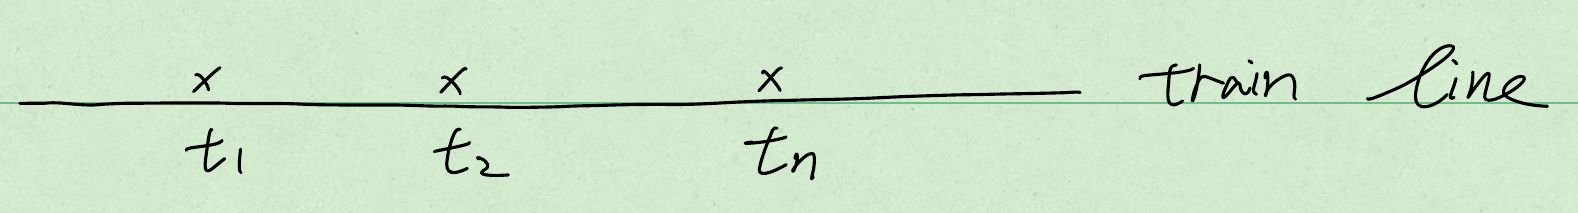
\includegraphics[width=0.5\textwidth]{fig/train-line.png}
\end{figure}

Greedy algorithm does not work for this problem. In greedy algorithm, unusually, we first find the set of town that must be served by the last station. Use greedy choice to identify that location and then recursively solve the problem. But we do not know how many town does the last station must serve and there is no obvious greedy strategy to answer this question.
 
Dynamic programming ask the same question, how many town should be served by the last station. But unlike greedy, since we do not know the answer, we try all the possible answers. 

Suppose the last station serves town $t_i, t_{i+1}, \cdots, t_n$ for some $i$. 

Notation: $C(n, k) = \text{cost of serving towns } t_1, \cdots, t_n$ with $k$ stations. Generally, $C(i, j)$ means the cost of serving towns $t_i, \cdots, t_j$ with $j$ station.

If someone told us that the optimal solution is for the last station to serve town $t_i^*, \cdots, t_n$, then 
\[C(n,k) = \max(\frac{t_n - t_i^*}{2}, ~C(i^* - 1, ~k - 1)).\]

Since we do not know $i$, we can write
\[C(n, k) = \min_{i = 1, \cdots, n}(\max(\frac{t_n - t_i}{2}, ~C(i -1, ~k - 1))).\]

Even though the number of sub-problems look like every big, there are actually only $n \times k$ kinds of problems.

\subsubsection{First algorithm}

Compute $C(n, k)$ exactly as in the recursion above.

\begin{algorithm}[H] 
	\caption{First Algorithm}
	\label{alg:loop}
	\begin{algorithmic}[1]
	\Require{n, k} \textbf{\textbf{}}
	\Ensure{Optimal Result}
	\Statex

%	\Comment{The g.c.d. of a and b}
	\Function{C}{$n,k$}
		\If {Base Cases}
			\State {$C(0, k \ge 0) = 0$}
			\State {$C(i, 1) = \frac{t_i - t_1}{2}$}
			\State {$C(i, i) = 0$}
		\Else
			\State {$min\_answer$ $\gets$ $\infty$}
			\For{$i \gets 1$ to $n$}      
			\If {$\max(\frac{t_n - t_i}{2},~C(i-1, k-1)) < min\_answer$}               
			\State {Update $min\_answer$}
			\EndIf
			\EndFor
			\State \Return {$min\_answer$}
		\EndIf
	\EndFunction
	\end{algorithmic}
\end{algorithm}

This recursive algorithm runs exponential time but we don't have too many distinct sub-problems. It is because we are solving the same sub-problems repeatedly.

Maintain solutions to solve sub-problems in a 2-D array. The C function, when called with argument $(i, j)$, first check if $C(i, j)$ is a known value in the array. If so, return it without any further call. So every sub-problem is solved only once. There are $n \times k$ sub-problems each take $O(n)$ time. It leads to a $O(n^2 k)$ algorithm.

Recall that we remember the answer of solved sub-problems and cutting short the recursion if the problem has been solved. This kind of techniques is called \textbf{memorization}.

